  \documentclass{article}

%\geometry{showframe}% for debugging purposes -- displays the margins

\newcommand{\E}{\mbox{E}}

\usepackage{amsmath}
\usepackage{enumitem}
\usepackage{amssymb}
\usepackage{fancyhdr} % Required for custom headers
\usepackage{lastpage} % Required to determine the last page for the footer
\usepackage{extramarks} % Required for headers and footers
\usepackage[usenames,dvipsnames]{color} % Required for custom colors
\usepackage{graphicx} % Required to insert images
\usepackage{listings} % Required for insertion of code
%\usepackage{couriernew} % Required for the courier font
\usepackage{amssymb}
\usepackage{algorithm2e}
\usepackage[noend]{algpseudocode}
\usepackage[thinlines]{easytable}
% \usepackage[letterpaper, landscape, margin=2in]{geometry}
\usepackage[a4paper, total={6in, 8in}]{geometry}


%\usepackage[garamond]{mathdesign}
\usepackage{url}

% Set up the images/graphics package
\usepackage{graphicx}
\setkeys{Gin}{width=\linewidth,totalheight=\textheight,keepaspectratio}
\graphicspath{{graphics/}}


\title{Amin Anvari}
\date{}
\author{SDS 385D - Statistical Models for Big Data\\ Assignment 1}

% \title[Exercises 1 $\cdot$ SDS 385]{Exercises 1: Preliminaries}
%\author[ ]{ }
\date{}  % if the \date{} command is left out, the current date will be used

% The following package makes prettier tables.  We're all about the bling!
\usepackage{booktabs}

% The units package provides nice, non-stacked fractions and better spacing
% for units.
\usepackage{units}

% The fancyvrb package lets us customize the formatting of verbatim
% environments.  We use a slightly smaller font.
\usepackage{fancyvrb}
\fvset{fontsize=\normalsize}

% Small sections of multiple columns
\usepackage{multicol}

% Provides paragraphs of dummy text
\usepackage{lipsum}

% These commands are used to pretty-print LaTeX commands
\newcommand{\doccmd}[1]{\texttt{\textbackslash#1}}% command name -- adds backslash automatically
\newcommand{\docopt}[1]{\ensuremath{\langle}\textrm{\textit{#1}}\ensuremath{\rangle}}% optional command argument
\newcommand{\docarg}[1]{\textrm{\textit{#1}}}% (required) command argument
\newenvironment{docspec}{\begin{quote}\noindent}{\end{quote}}% command specification environment
\newcommand{\docenv}[1]{\textsf{#1}}% environment name
\newcommand{\docpkg}[1]{\texttt{#1}}% package name
\newcommand{\doccls}[1]{\texttt{#1}}% document class name
\newcommand{\docclsopt}[1]{\texttt{#1}}% document class option name

\newcommand{\N}{\mbox{N}}
\newcommand{\thetahat}{\hat{\theta}}
\newcommand{\sigmahat}{\hat{\sigma}}
\newcommand{\betahat}{\hat{\beta}}


\begin{document}

% \maketitle% this prints the handout title, author, and date
\maketitle

\section{Linear regression}

Consider the simple linear regression model
$$
y = X \beta + e \, ,
$$
where $y = (y_1, \ldots, y_N)$ is an $N$-vector of responses, $X$ is an $N \times P$ matrix of features whose $i$th row is $x_i$, and $e$ is a vector of model residuals.  The goal is to estimate $\beta$, the unknown $P$-vector of regression coefficients.  

Let's say you trust the precision of some observations more than others, and therefore decide to estimate $\beta$ by the principle of weighted least squares (WLS):
$$
\hat{\beta} = \arg \min_{\beta \in \mathcal{R}^P} \sum_{i=1}^N \frac{w_i}{2}(y_i - x_i^T \beta)^2 \, ,
$$
where $w_i$ is the weight for observation $i$.  (Higher weight means more influence on the answer; the factor of 1/2 is just for convenience, as you'll see later.)

\begin{enumerate}[label=(\Alph*)]

\item Rewrite the WLS objective function\footnote{That is, the thing to be minimized.} above in terms of vectors and matrices, and show that $\hat \beta$ is the solution to the following linear system of $P$ equations in $P$ unknowns:
$$
(X^T W X) \hat \beta = X^T W y \, ,
$$
where $W$ is the diagonal matrix of weights.


\bigskip
{\color{blue}
Let's first write the (WLS) objective function in terms of vectors and matrices:
		\begin{align}
			\hat{\beta} &= \argmin_{\beta \in \mathbb{R}^p} \sum_{i=1}^{N} \frac{w_i}{2} \left ( y_i - x_i^T\beta \right )^2 \\
			&= \argmin_{\beta \in \mathbb{R}^p} \frac{1}{2} (y-X \beta)^T W (y-X\beta).
		\end{align}
		We can then expand this equation:
		\begin{align}
			\frac{1}{2} (y-X \beta)^T W (y-X\beta) &= \frac{1}{2} (y^T - \beta^T X^T)W(y-X\beta) \\
			&= \frac{1}{2} (y^TW - \beta^T X^TW)(y-X\beta) \\
			&= \frac{1}{2} (y^TWy -\beta^TX^TWy-y^TWX\beta + \beta^TX^TWX\beta) \\
			&= \frac{1}{2} (y^TWy - 2(X\beta)^TWy +\beta^TX^TWX\beta) \\
			&= \frac{1}{2} y^TWy - (X\beta)^TWy + \frac{1}{2} \beta^TX^TWX\beta, \label{eqn1}
		\end{align}

		To minimize the  objective function we take the gradient with respect to $\beta$ and set it equal to zero. 
		\begin{enumerate}
			\item % i
				\begin{align}
					\nabla_{\beta}( \frac{1}{2} y^TWy )= 0
				\end{align}
			\item % ii
				\begin{align}
					\nabla_{\beta} (-(X\beta)^TWy) = - X^TWy
				\end{align}
			\item % iii
				\begin{align}
					\nabla_{\beta} (\frac{1}{2} \beta^TX^TWX\beta) &= \frac{1}{2} \beta^T (X^TWX + (X^TWX)^T) \\
					&= X^TWX\beta.
				\end{align}
		\end{enumerate}
		We have to sum all these three terms and set it equal to zero:
            \begin{align}
			X^TWX\beta - X^TWy &= 0 \implies
			 (X^TWX)\hat{\beta} = X^TWy
			 \end{align}


}






\item One way to calculate $\hat{\beta}$ is to: (1) recognize that, trivially, the solution to the above linear system must satisfy $\hat \beta = (X^T W X)^{-1} X^T W y$; and (2) to calculate this directly, i.e.~by inverting $X^T W X$.  Let's call this the ``inversion method'' for calculating the WLS solution.


Numerically speaking, is the inversion method the fastest and most stable way to actually solve the above linear system?  Do some independent sleuthing on this question.  Summarize what you find, and provide pseudo-code for at least one alternate method based on matrix factorizations---call it ``your method'' for short.  (Note: our linear system is not a special flower; whatever you discover about general linear systems should apply here.)

\bigskip
{\color{blue}
solving Eqn. (12) using the inversion method yields:
		\begin{align}
			\hat{\beta} = (X^TWX)^{-1}X^TWy.
		\end{align} 
		Inverting a matrix in general is a no no! it is very expensive
		to invert a matrix in general. It is also not a stable method of
		solving linear systems. Cholesky factorization, QR factorization, and singular value decomposition are three alternative way that we can solve the WLS equation. Here we discuss Cholesky Decomposition to solve WLS.\\

			\textbf{Cholesky Decomposition Method:} \\
			Let 
			\begin{align}
				C = X^TWX, \;\;D=X^TWy
			\end{align}
			so 
			\begin{align}
				C\hat{\beta} = D.
			\end{align}
			Matrix $C$ can be decomposed into a lower-triangular matrix and an upper-triangular matrix, such that $U=L^T$ so
			\begin{align}
				C &= LU = LL^T \implies 
				LL^T\hat{\beta} = D.
			\end{align}
			Let's define matrix $M = L^T\hat{\beta}$. The problem changed into solving two much simpler problems. 
			\begin{align}
				LM &= D \\
				L^T\hat{\beta} &= M
			\end{align}
			
			Here both L and U are triangular and therefore solving these two equations are much less expensive. Therefore, this method 
			is a much better way of solving the system by taking advantage of the symmetry of the matrix.
		
		Cholesky decomposition method:\\
			\begin{algorithm}[H]
			 \{ \\
			 \vspace{2mm}
			 Compute $D = X^T W y$ \; 
			 Compute $C = X^T W X$\; 
			 \vspace{2mm}
			 Compute $U$ as the upper triangular matrix from Cholesky decomposition of $C$\;
			 Compute $L = U^T$\; 
			 \vspace{2mm}
			 Solve for $M$ in $LM=D$\;
			 Solve for $\hat{\beta}$ in $L^T\hat{\beta}=U\hat{\beta}=M$\;
			 \vspace{2mm}
			 return$(\hat{\beta}$)\; 
			 \}
			 \caption{Cholesky Decomposition Algorithms}
			\end{algorithm}


}

\clearpage
\item Code up functions that implement both the inversion method and your method for an arbitrary $X$, $y$, and weights $W$.  Obviously you shouldn't write your own linear algebra routines for doing things like multiplying or decomposing matrices, but don't use a direct model-fitting function like R's ``lm'' either.   Your actual code should look a lot like the pseudo-code you wrote for the previous part.  Note: be attentive to how you multiply a matrix by a diagonal matrix, or you'll waste a lot of time multiplying stuff by zero.

Now simulate some silly data from the linear model for a range of values of $N$ and $P$.  (Feel free to assume that the weights $w_i$ are all 1.)  It doesn't matter how you do this---e.g.~everything can be Gaussian if you want.  (We're not concerned with statistical principles yet, just with algorithms, and using least squares is a pretty terrible idea for enormous linear models, anyway.)  Just make sure that you explore values of $P$ up into the thousands, and that $N > P$.  Benchmark the performance of the inversion solver and your solver across a range of scenarios.  (In R, a simple library for this purpose is microbenchmark.)

\item Now what happens if $X$ is a highly sparse matrix, in the sense that most entries are zero?  Ideally we'd realize some savings by not doing a whole bunch of needless multiplication by zero in our code.

It's easy to simulate an $X$ matrix that looks like this.  A quick-and-dirty way is to simulate a mask of zeros and ones (but mostly zeros), and then do pointwise multiplication with your original feature matrix.  For example:
\begin{verbatim}
N = 2000
P = 500
X = matrix(rnorm(N*P), nrow=N)
mask = matrix(rbinom(N*P,1,0.05), nrow=N)
X = mask*X
X[1:10, 1:10]  # quick visual check
\end{verbatim}

Again assume that the weights $w_i$ are all 1.  Repeat the previous benchmarking exercise with this new recipe for simulating a sparse $X$, except add another solver to the mix: one that can solve a linear system $Ax = b$ in a way that exploits the sparsity of A.  To do this, you'll need to actually represent the feature matrix $X$ in a sparse format, and then call the appropriate routines  for that format.  (Again, do some sleuthing; in R, the Matrix library has data structures and functions that can do this; SciPy will have an equivalent.)

Benchmark the inversion method, your method, and the sparse method across some different scenarios (including different sparsity levels in $X$, e.g. 5\% dense in my code above).
\end{enumerate}


\section{Generalized linear models}

As an archetypal case of a GLM, we'll consider the binomial logistic regression model: $y_i \sim \mbox{Binomial}(m_i, w_i)$, where $y_i$ in an integer number of ``successes,'' $m_i$ is the number of trials for the $i$th case, and the success probability $w_i$ is a regression on a feature vector $x_i$ given by the inverse logit transform:
$$
w_i = \frac{1}{1 + \exp\{-x_i^T \beta\}} \, .
$$
We want to estimate $\beta$ by the principle of maximum likelihood.  Note: for binary logistic regression, $m_i = 1$ and $y_i$ is either 0 or 1.

As an aside, if you have a favorite data set or problem that involves a different GLM---say, a Poisson regression for count data---then feel free to work with that model instead throughout this entire section.  The fact that we're working with a logistic regression isn't essential here; any GLM will do.

\begin{enumerate}[label=(\Alph*)]
\item Start by writing out the negative log likelihood,
$$
l(\beta) = - \log \left \{ \prod_{i=1}^N p(y_i \mid \beta) \right \} \, .
$$
Simplify your expression as much as possible. This is the thing we want to minimize to compute the MLE.  (By longstanding convention, we phrase optimization problems as minimization problems.)

Derive the gradient of this expression, $\nabla l(\beta)$.   Note: your gradient will be a sum of terms $l_i(\beta)$, and it's OK to use the shorthand
$$
w_i(\beta) =  \frac{1}{1 + \exp\{-x_i^T \beta\}}
$$
in your expression.

\bigskip
{\color{blue}
We have $y_i \sim \text{Binomial}(m_i, w_i)$, where 
	\begin{align}
		w_i = \frac{1}{1+\exp(-x_i^T\beta)}, \;\; 1-w_i = \frac{\exp(-x_i^T\beta)}{1+\exp(-x_i^T\beta)},
	\end{align}
	so the negative log likelihood is
	%
	%
	%
	% LOG LIK FN
	%
	%
	%
	\begin{align}
		\ell(\beta) &= -\log \left \{ \prod_{i=1}^N p(y_i | \beta)  \right \} \\
		&= -\log \left \{ \prod_{i=1}^N \binom {m_i}{y_i}(w_i)^{y_i}(1-w_i)^{m_i-y_i}  \right \} \\
		&= - \left \{ \sum_{i=1}^{N} \left ( \log\binom {m_i}{y_i} + y_i \log(w_i) + (m_i-y_i)\log(1-w_i) \right ) \right \} \\
		&= - \left \{ \sum_{i=1}^{N} \left ( \log\binom {m_i}{y_i} + y_i \log\left ( \frac{1}{1+\exp(-x_i^T\beta)} \right ) + (m_i-y_i)\log\left ( \frac{\exp(-x_i^T\beta)}{1+\exp(-x_i^T\beta)} \right) \right ) \right \} \\
		& = - \left \{ \sum_{i=1}^{N} \left ( \log\binom {m_i}{y_i} - y_i\log(1+\exp(-x_i^T\beta)) - (m_i-y_i)x_i^T\beta \\& -m_i\log(1+\exp(-x_i^T\beta)) + y_i\log(1+\exp(-x_i^T\beta)) \right ) \right \} \\
		& = - \left \{ \sum_{i=1}^{N} \left ( \log\binom {m_i}{y_i} - (m_i-y_i)x_i^T\beta -m_i\log(1+\exp(-x_i^T\beta)) \right ) \right \} \\
		& = \sum_{i=1}^{N} \left ((m_i-y_i)x_i^T\beta +m_i\log(1+\exp(-x_i^T\beta)) - \log\binom {m_i}{y_i} \right ) \label{finalll}
		%%%
		%%%
		%%%
	\end{align}
	The gradient for this expression is, 
	%
	%
	%
	% GRAD FN
	%
	%
	%
	\begin{align}
		\nabla \ell (\beta) &= \sum_{i=1}^N \left ( (m_i-y_i)x_i - m_i \frac{\exp({-x_i^T\beta})}{1+\exp(-x_i^T\beta)}x_i \right ) \\
		&= \sum_{i=1}^N \left ( (m_i-y_i)x_i - m_i (1-w_i)x_i \right ) \\
		&= \sum_{i=1}^N (m_iw_i-y_i)x_i \\
		&= -X^T(y-mw)
	\end{align}
	where $y$ is the $n \times 1$ vector of responses and $mw$ is the element-wise product of the two $n \times 1$ vectors $m$ and $w$.

}

\item Read up on the method of steepest descent, i.e.~gradient descent, in Nocedal and Wright (see course website).  Write your own function that will fit a logistic regression model by gradient descent.  Grab the data ``wdbc.csv'' from the course website, or obtain some other real data that interests you, and test it out.  The WDBC file has information on 569 breast-cancer patients from a study done in Wisconsin.  The first column is a patient ID, the second column is a classification of a breast cell (Malignant or Benign), and the next 30 columns are measurements computed from a digitized image of the cell nucleus.  These are things like radius, smoothness, etc.  For this problem, use the first 10 features for $X$, i.e.~columns 3-12 of the file.  If you use all 30 features you'll run into trouble.

Some notes here:
\begin{enumerate}
\item You can handle the intercept/offset term by either adding a column of 1's to the feature matrix $X$, or by explicitly introducing an intercept into the linear predictor and handling the intercept and regression coefficients separately, i.e.
$$
w_i(\beta) =  \frac{1}{1 + \exp\{-(\alpha + x_i^T \beta )\}} \, .
$$
\item I strongly recommend that you write a self-contained function that, for given values of $\beta$, $y$, $X$, and sample sizes $m_i$ (which for the WDBC data are all 1), will calculate the gradient of $l(\beta)$.  Your gradient-descent optimizer will then call this function.  Modular code is reusable code.
\item Make sure that, at every iteration of gradient descent, you compute and store the current value of the log likelihood, so that you can track and plot the convergence of the algorithm.
\item Be sensitive to the numerical consequences of an estimated success probability that is either very near 0, or very near 1.
\item Finally, you can be as clever as you want about the gradient-descent step size.  Small step sizes will be more robust but slower; larger step sizes can be faster but may overshoot and diverge; step sizes based on line search (Chapter 3 of Nocedal and Wright) are cool but involve some extra work.
\end{enumerate}


\item Now consider a point $\beta_0 \in \mathcal{R}^P$, which serves as an intermediate guess for our vector of regression coefficients.  Show that the second-order Taylor approximation of $l(\beta)$, around the point $\beta_0$, takes the form
$$
q(\beta; \beta_0) = \frac{1}{2}(z - X \beta)^T W (z - X \beta) + c\, ,
$$
where $z$ is a vector of ``working responses'' and $W$ is a diagonal matrix of ``working weights,'' and $c$ is a constant that doesn't involve $\beta$.  Give explicit expressions for the diagonal elements $W_{ii}$ and for $z_i$ (which will necessarily involve the point $\beta_0$, around which you're doing the expansion).\footnote{Remember the trick of completing the square, e.g.~\url{https://justindomke.wordpress.com/completing-the-square-in-n-dimensions/}.}

{\color{blue}
We need to calculate the Hessian matrix of the log likelihood function, $\nabla^2 \ell(\beta) $. The Hessian will be a $P\times P$ matrix, with the element in row $i$ and column $j$ being:
	\begin{align}
		\frac{\partial^2}{\partial \beta_i \partial \beta _j}\ell (\beta) &= \frac{\partial}{\partial \beta_i} \left ( \frac{\partial}{\partial \beta_j} \ell (\beta) \right ) \\
		&= \frac{\partial}{\partial \beta_i} \left ( \frac{\partial}{\partial \beta_j} \sum_{k=1}^N \left [(m_k-y_k)x_i^T\beta +m_k\log(1+\exp(-x_k^T\beta)) - \log\binom {m_k}{y_k} \right ] \right ) \\
		&= \frac{\partial}{\partial \beta_i} \left ( \nabla_j \ell(\beta) \right ) \\
		&= \frac{\partial}{\partial \beta_i} \left ( \sum_{k=1}^N(m_kw_k-y_k)x_{kj} \right )  \\
		&= \sum_{k=1}^{N} x_{ki}x_{kj}m_k w_k(1-w_k)
	\end{align}
	Note: 
	\begin{align}
		\frac{\partial}{\partial \beta_i} w_k &= x_{ki} \frac{\exp(-x_k^T\beta)}{(1+\exp(-x_k^T\beta))^2} \\
		&= x_{ki} w_k(1-w_k)
	\end{align}
	This matrix is equivalent to $X^TWX$ where $W = \text{diag}(m_1w_1(1-w_1),\ldots, m_Nw_N(1-w_N))$ \\
	
	Let $a = (y-mw)$. We have already shown that $\nabla \ell(\beta) = -X^T (y-mw) = -X^T a$ and $\nabla^2 \ell (\beta) = X^T W X$. The second-order Taylor approximation for $\ell(\beta)$ around the point $\beta_0$ is,
	%
	%
	%
	% Taylor approx
	%
	%
	%
	\begin{align}
		\hat{\ell}(\beta) &= \ell(\beta_0)+(\nabla \ell(\beta))^T(\beta-\beta_0) + \frac{1}{2}(\beta-\beta_0)^T \nabla^2 \ell(\beta) (\beta-\beta_0) \\
		&= \ell(\beta_0) + (-X^T a)^T(\beta - \beta_0) + \frac{1}{2}(\beta - \beta_0)^T X^T W X (\beta - \beta_0) \\
		&= \frac{1}{2} ( [ \beta - \beta_0 ] -(X^T W X)^{-1} X^T a )^T X^T W X ( [ \beta - \beta_0 ] -(X^T W X)^{-1} X^T a ) + c \\ 
		&= \frac{1}{2} (\beta - \beta_0  + X^{-1}W^{-1}(X^T)^{-1}X^T a )^T X^T W X (\beta - \beta_0 + X^{-1}W^{-1}(X^T)^{-1}X^T a ) + c \\
		&= \frac{1}{2} (\beta - \beta_0 + X^{-1}W^{-1} a )^T X^T W X (\beta - \beta_0 X^{-1}W^{-1} a ) + c \\
		&= \frac{1}{2} (X\beta - X\beta_0 + XX^{-1}W^{-1} a )^T W (X\beta - X\beta_0 + X X^{-1}W^{-1} a ) + c \\
		&= \frac{1}{2} (X\beta - X\beta_0 + W^{-1} a )^T W (X\beta - X\beta_0 + W^{-1} a ) + \ldots \\
		&= \frac{1}{2}(z-X\beta)^T W (z-X\beta) + c,
	\end{align}
	where $c$ is some constant, $z = X\beta_0 + W^{-1}a = X\beta_0 + W^{-1}(y-mw)$
%%
%%
%%
%%
%%
}


\item Read up on Newton's method in Nocedal and Wright, Chapter 2.  Implement it for the logit model and test it out on the same data set you just used to test out gradient descent.\footnote{You should be able to use your own solver for linear systems from the first section.}  Note: while you could do line search, there is a ``natural'' step size of 1 in Newton's method.

{\color{blue}

Now we use Newton's to estimate $\beta$. This is also an iterative process, though now we need far fewer iterations to achieve convergence because we are taking the curvature of our objective function ($\ell(\beta)$) into account. In fact, we only use 10 iterations and achieve estimates $\hat{\beta}$ which are \emph{exactly} in line with estimates from \texttt{glm}. \\
\textbf{Newton's Method:} 
\begin{align}
	\hat{\beta}_{t+1} = \hat{\beta}_t - (\nabla^2\ell(\hat{\beta}_t))^{-1}\nabla\ell(\hat{\beta_t})
\end{align}
		\begin{figure}[htp!]
		\centering
			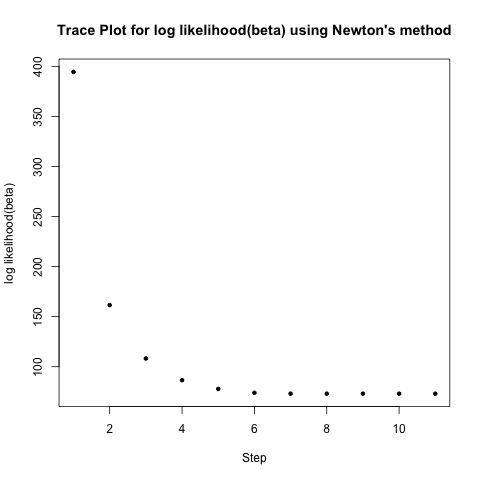
\includegraphics[scale=0.5]{beta_newton.png}
			\caption{Log likelihood trace plot for Newton's method}
		\end{figure}
\begin{figure}[htp!]
		\centering
		\label{my-label2}
		\begin{tabular}{l|r|r}
		                        & N.'s method & R: \texttt{glm} \\ \hline
								\\[-1em]
		$\hat{\beta}_1$      & 0.48702           & 0.48702         \\  \hline
		\\[-1em]
		$\hat{\beta}_2$      & -7.22185          & -7.22185         \\ \hline
		\\[-1em]
		$\hat{\beta}_3$      & 1.65476          & 1.65476         \\ \hline
		\\[-1em]
		$\hat{\beta}_4$      & -1.73763           & -1.73763        \\ \hline
		\\[-1em]
		$\hat{\beta}_5$      & 14.00485        & 14.00485        \\ \hline
		\\[-1em]
		$\hat{\beta}_6$      & 1.07495             & 1.07495         \\ \hline
		\\[-1em]
		$\hat{\beta}_7$      & -0.07723          & -0.07723        \\ \hline
		\\[-1em]
		$\hat{\beta}_8$      & 0.67512            & 0.67512         \\ \hline
		\\[-1em]
		$\hat{\beta}_9$      & 2.59287         & 2.59287         \\ \hline
		\\[-1em]
		$\hat{\beta}_{10}$ & 0.44626          & 0.44626         \\ \hline
		\\[-1em]
		$\hat{\beta}_{11}$ & -0.48248           & -0.48248           
		\end{tabular}
		\caption{Comparison of results from Newton's method and \texttt{glm}}
	\end{figure}
%%
%%
%%
%%
%%
}


\pagebreak
\item Reflect broadly on the tradeoffs inherent in the decision of whether to use gradient descent or Newton's method for solving a logistic-regression problem.

{\color{blue}
Gradient descent requires many iterations, and there is no simple way to know what step size is wise, or even to know just how many iterations are sufficient to reach convergence. The only way to find out is to experiment with different numbers of iterations and step sizes. In contrast, Newton's method converges upon the MLE with far fewer iterations because we are using knowledge of the ``curvature" of our function to be minimized. However, for Newton's method we must invert the Hessian matrix, which is computationally intensive for large matrices, and potentially unstable, leaving us vulnerable to floating point errors. It also possible that the Hessian matrix has no closed form solution or is so convoluted as to make its computation difficult.
%%
%%
%%
%%
%%
}



\end{enumerate}


\end{document}




